\documentclass{article}

\usepackage{amsmath, amssymb}
\usepackage{graphicx}

\title{Time and Distance}
\author{Richard Feynman}
\begin{document}

	\maketitle

	\section{Short distances}

	Now let’s think about smaller distances. Subdividing the meter is easy. Without much difficulty we can mark off one thousand equal spaces which add up to one meter. With somewhat more difficulty, but in a similar way (using a good microscope), we can mark off a thousand equal subdivisions of the millimeter to make a scale of microns (millionths of a meter). It is difficult to continue to smaller scales, because we cannot “see” objects smaller than the wavelength of visible light (about $5 \times 10^{-7}$ meter).\\

	\begin{figure}[h]
	\centering
		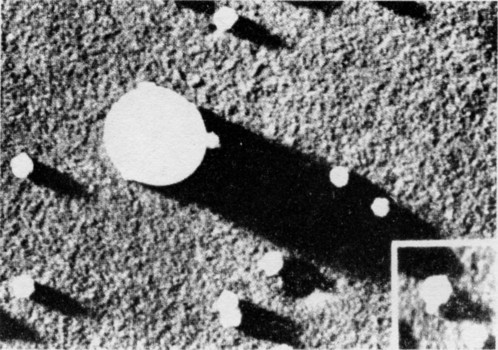
\includegraphics[scale=2.0]{img1.png}
		\caption{Electron micrograph of some virus molecules. The “large” sphere is for calibration and is known to have a diameter of $2 \times 10^{-7}$ meter (2000 A).}
		\label{Fi: Img59}
	\end{figure}

	We need not stop, however, at what we can see. With an electron microscope, we can continue the process by making photographs on a still smaller scale, say down to $10^{-8}$ meter (Fig \ref{Fi: Img59}). By indirect measurements by a kind of triangulation on a microscopic scale we can continue to measure to smaller and smaller scales. First, from an observation of the way light of short wavelength (x-radiation) is reflected from a pattern of marks of known separation, we determine the wavelength of the light vibrations. Then, from the pattern of the scattering of the same light from a crystal, we can determine the relative location of the atoms in the crystal, obtaining results which agree with the atomic spacings also determined by chemical means. We find in this way that atoms have a diameter of about $10^{-10}$ meter.\\ 

	There is a large “gap” in physical sizes between the typical atomic dimension of about $10^{-10}$ meter and the nuclear dimensions $10^{-15}$ meter, $10^{-5}$ times smaller. For nuclear sizes, a different way of measuring size becomes convenient. We measure the apparent area, σ, called the effective cross section. If we wish the radius, we can obtain it from $\sigma = \phi r^{2}$, since nuclei are nearly spherical.\\

	Measurement of a nuclear cross section can be made by passing a beam of high-energy particles through a thin slab of material and observing the number of particles which do not get through. These high-energy particles will plow right through the thin cloud of electrons and will be stopped or deflected only if they hit the concentrated weight of a nucleus. Suppose we have a piece of material 1 centimeter thick. There will be about $10^{-8}$ atomic layers. But the nuclei are so small that there is little chance that any nucleus will lie behind another. We might imagine that a highly magnified view of the situation—looking along the particle beam—would look like Fig \ref{Fi: Img60}.\\ 

	\begin{figure}[h]
	\centering
		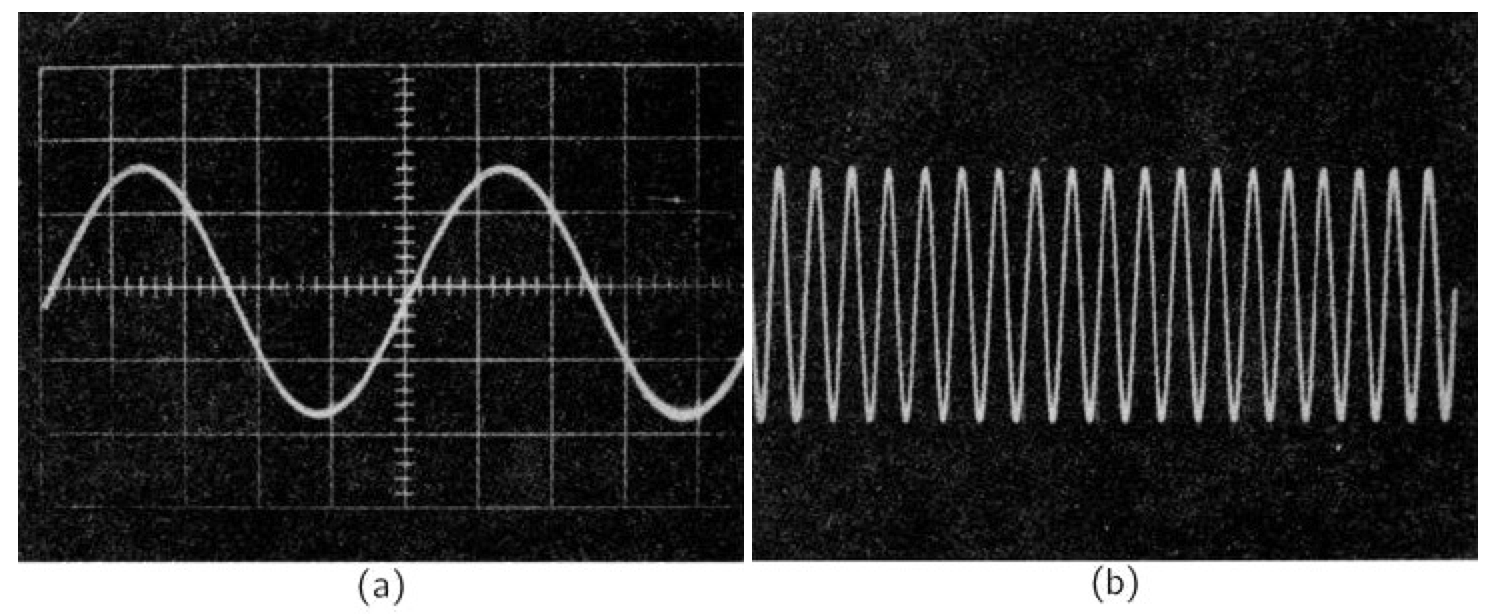
\includegraphics[scale=2.0]{img2.png}
		\caption{Imagined view through a block of carbon 1 cm thick if only the nuclei were observed.}
		\label{Fi: Img60}
	\end{figure}

	The chance that a very small particle will hit a nucleus on the trip through is just the total area covered by the profiles of the nuclei divided by the total area in the picture. Suppose that we know that in an area A of our slab of material there are N atoms (each with one nucleus, of course). Then the fraction of the area “covered” by the nuclei is $\frac{N \sigma}{A}$. Now let the number of particles of our beam which arrive at the slab be n1 and the number which come out the other side be n2. The fraction which do not get through is $\frac{n_{1} - n_{2}}{n_{1}}$, which should just equal the fraction of the area covered. We can obtain the radius of the nucleus from the equation \ref{Equ1}.\\

	\begin{equation}
	\centering
		\phi r^{2} = \sigma = \frac{A}{N} \frac{n_{1} - n_{2}}{n_{1}}
		\label{Equ1}
	\end{equation}

	From such an experiment we find that the radii of the nuclei are from about 1 to 6 times $10^{-15}$ meter. The length unit $10^{-15}$ meter is called the fermi, in honor of Enrico Fermi (1901–1954).\\

	What do we find if we go to smaller distances? Can we measure smaller distances? Such questions are not yet answerable. It has been suggested that the still unsolved mystery of nuclear forces may be unravelled only by some modification of our idea of space, or measurement, at such small distances.\\

	\begin{table}[h] % Para poner en el lugar de definicion
	\centering
		\begin{tabular}{| l | c | c | c}
			\hline
			Nombre & Primero & Secundo \\ \hline
			Ana & 5.0 & 3.4 \\ \hline
			Beatriz & 4.2 & 2.4 \\ \hline
			Carlos & 3.4 & 5.0 \\ \hline
		\end{tabular}
	\caption{Notas de los parciales}
	\label{Ta: Notas}
	\end{table}

	It might be thought that it would be a good idea to use some natural length as our unit of length—say the radius of the earth or some fraction of it. The meter was originally intended to be such a unit and was defined to be $(\phi / 2) \times 10^{7}$ times the earth’s radius. It is neither convenient nor very accurate to determine the unit of length in this way. For a long time it has been agreed internationally that the meter would be defined as the distance between two scratches on a bar kept in a special laboratory in France. More recently, it has been realized that this definition is neither as precise as would be useful, nor as permanent or universal as one would like. It is currently being considered that a new definition be adopted, an agreed-upon (arbitrary) number of wavelengths of a chosen spectral line.\\ 

	Measurements of distance and of time give results which depend on the observer. Two observers moving with respect to each other will not measure the same distances and times when measuring what appear to be the same things. Distances and time intervals have different magnitudes, depending on the coordinate system (or “frame of reference”) used for making the measurements. We shall study this subject in more detail in a later chapter.\\ 

	Perfectly precise measurements of distances or times are not permitted by the laws of nature. We have mentioned earlier that the errors in a measurement of the position of an object must be at least as large as:

	$$\bigtriangleup x \geq \hbar / 2 \bigtriangleup p $$

	where $\hbar$ is a small fundamental physical constant called the reduced Planck constant and $\bigtriangleup p$ is the error in our knowledge of the momentum (mass times velocity) of the object whose position we are measuring. It was also mentioned that the uncertainty in position measurements is related to the wave nature of particles.

	The relativity of space and time implies that time measurements have also a minimum error, given in fact by:

	$$\bigtriangleup t \geq \hbar / 2 \bigtriangleup E $$

	where $\bigtriangleup E$ is the error in our knowledge of the energy of the process whose time period we are measuring. If we wish to know more precisely when something happened we must know less about what happened, because our knowledge of the energy involved will be less. The time uncertainty is also related to the wave nature of matter. 


\end{document}